\documentclass[10pt]{article}

\usepackage[margin=0.62in,headheight=14pt,footskip=24pt]{geometry}
\usepackage[T1]{fontenc}
\usepackage{lmodern}
\usepackage{microtype}
\usepackage{xcolor}
\usepackage{tabularx}
\usepackage{booktabs}
\usepackage{enumitem}
\usepackage{tikz}
\usepackage{graphicx}
\usepackage{fancyhdr}
\usepackage{titlesec}
\usepackage{hyperref}
\usetikzlibrary{positioning,arrows.meta}

\definecolor{ink}{HTML}{17243A}
\definecolor{indigo}{HTML}{3545A5}
\definecolor{pale}{HTML}{EEF1FF}
\definecolor{muted}{HTML}{58667A}
\definecolor{amber}{HTML}{8A5B00}
\definecolor{line}{HTML}{D7DDE7}

\hypersetup{colorlinks=true,linkcolor=indigo,urlcolor=indigo}
\pagestyle{fancy}
\fancyhf{}
\fancyhead[L]{\small\textcolor{muted}{COVENANT INTELLIGENCE}}
\fancyhead[R]{\small\textcolor{muted}{TRESATA TAKE-HOME}}
\fancyfoot[L]{\small\textcolor{muted}{Synthetic-data prototype; not legal advice}}
\fancyfoot[R]{\small\textcolor{muted}{\thepage}}
\setlength{\parindent}{0pt}
\setlength{\parskip}{4pt}
\setlist[itemize]{leftmargin=1.2em,itemsep=2pt,topsep=2pt}
\setlist[enumerate]{leftmargin=1.35em,itemsep=2pt,topsep=2pt}
\titleformat{\section}{\large\bfseries\color{ink}}{}{0pt}{}
\titlespacing*{\section}{0pt}{8pt}{3pt}
\titleformat{\subsection}{\normalsize\bfseries\color{indigo}}{}{0pt}{}
\titlespacing*{\subsection}{0pt}{5pt}{2pt}

\newcommand{\eyebrow}[1]{\textcolor{indigo}{\small\bfseries\MakeUppercase{#1}}}
\newcommand{\callout}[1]{\noindent\colorbox{pale}{\parbox{\dimexpr\linewidth-2\fboxsep}{#1}}}
\newcommand{\smallnote}[1]{\textcolor{muted}{\small #1}}
\newcommand{\riskrow}[2]{\textbf{#1} & #2\\}

\begin{document}

% PAGE 1 - PROBLEM
\eyebrow{Corporate finance | Problem brief}
\vspace{3pt}
{\LARGE\bfseries\color{ink} From credit agreement clauses to an auditable obligation register}\par
\vspace{3pt}
{\large\color{muted} Covenant Intelligence helps treasury teams turn long-form loan terms into reviewable obligations and a quarterly tracker.}\par
\vspace{7pt}
\callout{\textbf{Problem statement.} Corporate treasurers and finance teams must find financial tests, reporting duties, deadlines, and restrictions in lengthy credit agreements, then keep them current as amendments arrive. The work is recurring and cross-referenced; a missed deadline or misunderstood clause can create avoidable compliance and financing risk.}

\section{The problem and why it matters}
The source of truth is usually prose spread across an agreement: the operative clause may depend on a defined term elsewhere, an exception, a measurement period, or another section. Teams must translate that language into calendar events, evidence requests, review steps, and amendment updates. Existing spreadsheets can track known tasks, but they do not reliably establish where each task came from or whether a later amendment changed it.

\begin{tabularx}{\linewidth}{@{}>{\bfseries}p{1.35in}X@{}}
\toprule
Who & Corporate treasury, finance directors, corporate finance, and compliance teams.\\
Task & Identify and maintain covenant tests, reporting obligations, negative restrictions, deadlines, conditions, and exceptions.\\
Cadence & Monitoring commonly recurs each fiscal quarter or year; reporting deadlines depend on each agreement.\\
Cost today & No defensible time or error-cost baseline has been measured for this prototype. A pilot should measure review time and correction rates rather than invent savings.\\
\bottomrule
\end{tabularx}

\section{Why now - and what is out of scope}
Language models can help locate and structure obligations expressed in varied prose, but producing plausible JSON is not the hard part. The hard part is preserving evidence, uncertainty, and human accountability while the underlying agreement changes. The prototype uses AI for drafting candidates and ordinary software for source handling, deterministic validation, persistence, status tracking, and audit history.

\begin{minipage}[t]{0.48\linewidth}
\textbf{In scope}
\begin{itemize}
  \item Page-level PDF text extraction and versioned source files.
  \item Evidence-backed draft obligations and human correction.
  \item Approved register, quarterly tracking, amendment proposals, and audit history.
\end{itemize}
\end{minipage}\hfill
\begin{minipage}[t]{0.48\linewidth}
\textbf{Out of scope}
\begin{itemize}
  \item Calculating financial ratios or covenant headroom.
  \item ERP integrations, autonomous approval, or binding legal advice.
  \item Private agreements in examples or evaluation; OCR for scanned pages.
\end{itemize}
\end{minipage}

\section{Pilot boundary}
Begin with public or synthetic credit agreements and a single workspace. The prototype does not assume a jurisdiction-specific legal interpretation. A qualified reviewer remains accountable for decisions and for translating approved obligations into the organization's operating process.

\newpage
% PAGE 2 - SOLUTION AND ARCHITECTURE
\eyebrow{Solution | How a document becomes a reviewed obligation}
\section{A draft-first workflow}
The user uploads an agreement version. PyMuPDF extracts text page by page and preserves page numbering and hashes. The backend splits nonblank text into bounded, page-mapped chunks and sends the full text to the configured OpenRouter model; lexical screening is disabled because a keyword list cannot reliably prove that unfamiliar contract language is irrelevant. The model proposes canonical obligation objects with wording, thresholds, periods, deadlines, definitions, cross-references, evidence, and uncertainty reasons.

Deterministic checks validate the JSON schema, required evidence shape, cited page existence, and whether each quoted passage appears in the cited page text. These checks prove traceability, not legal correctness. A reviewer then inspects the original PDF, corrects or rejects candidates, and approves only a complete validated obligation. Approval creates a new revision; it never overwrites the original model candidate.

\begin{center}
\resizebox{\linewidth}{!}{%
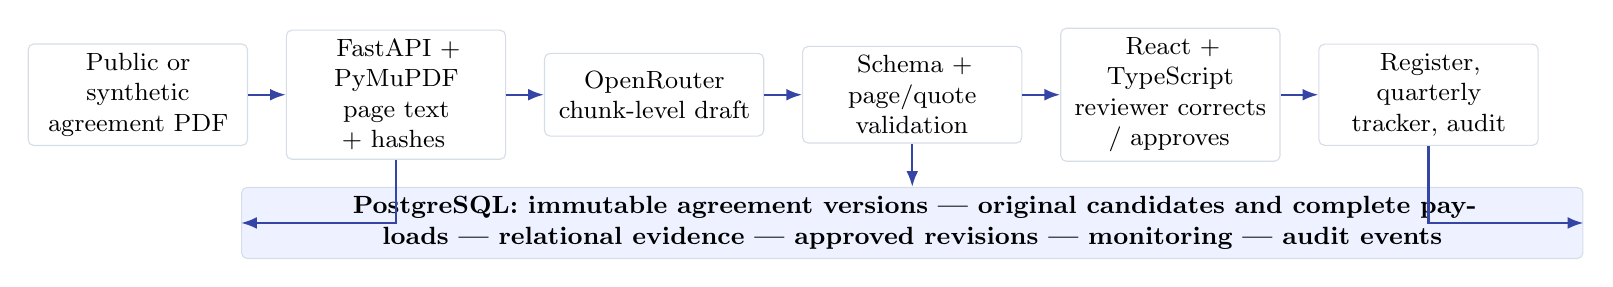
\begin{tikzpicture}[
  box/.style={draw=line,rounded corners=2pt,fill=white,align=center,
    text width=2.55cm,minimum height=1.05cm,font=\small},
  flow/.style={-{Latex[length=2mm]},draw=indigo,line width=0.8pt},
  store/.style={draw=line,rounded corners=2pt,fill=pale,align=center,
    text width=16.8cm,minimum height=0.72cm,font=\small\bfseries}
]
\node[box] (pdf) {Public or synthetic\\agreement PDF};
\node[box,right=0.48cm of pdf] (text) {FastAPI + PyMuPDF\\page text + hashes};
\node[box,right=0.48cm of text] (ai) {OpenRouter\\chunk-level draft};
\node[box,right=0.48cm of ai] (check) {Schema + page/quote\\validation};
\node[box,right=0.48cm of check] (human) {React + TypeScript\\reviewer corrects / approves};
\node[box,right=0.48cm of human] (track) {Register, quarterly\\tracker, audit};
\draw[flow] (pdf) -- (text);
\draw[flow] (text) -- (ai);
\draw[flow] (ai) -- (check);
\draw[flow] (check) -- (human);
\draw[flow] (human) -- (track);
\node[store,below=0.55cm of check] (db) {PostgreSQL: immutable agreement versions | original candidates and complete payloads | relational evidence | approved revisions | monitoring | audit events};
\draw[flow] (text.south) |- (db.west);
\draw[flow] (check.south) -- (db.north);
\draw[flow] (track.south) |- (db.east);
\end{tikzpicture}%
}
\end{center}

\section{Why AI - and what it must not decide}
Simple keyword rules are brittle when clauses use uncommon wording, split requirements across pages, or rely on definitions and exceptions. An LLM can propose candidate interpretations across these patterns. It does not establish truth: validation and review determine whether a draft can enter the approved register. Ratios are recorded as written, not calculated. Due dates are configured only when the agreement supports the rule; ambiguity remains unresolved for a person.

\callout{\textbf{Core trust rule.} Every candidate carries source wording and page-level evidence. A model confidence score is not evidence. An empty model response is not proof that the agreement contains no obligations.}

\newpage
% PAGE 3 - SYSTEM DESIGN AND DATA
\eyebrow{System design | Keep probabilistic and exact work apart}
\section{Modular monolith, explicit boundaries}
The MVP uses a React + TypeScript + Tailwind frontend and a Python FastAPI backend. Backend modules separate PDF ingestion, extraction/provider integration, validation, workflow logic, and persistence. PostgreSQL stores workspace-scoped records; SQLAlchemy and Alembic provide persistence and migrations. OpenRouter sits behind an OpenAI-compatible provider adapter. This is one deployable application with clear module seams, not a collection of services or autonomous agents.

\begin{tabularx}{\linewidth}{@{}p{1.6in}XX@{}}
\toprule
Concern & AI-assisted / probabilistic & Deterministic / accountable\\
\midrule
Finding obligations & Interpret varied clause wording and suggest a structured draft. & Requested categories, document version, page map, and chunk coverage are recorded.\\
Thresholds and dates & Extract values and preserve rule wording; flag ambiguity. & Do not calculate ratios. Do not infer missing values or dates.\\
Definitions & Suggest relevant definitions and references. & Resolve only against supplied agreement pages; retain unresolved references as uncertainty.\\
Evidence & Suggest supporting passages. & Validate cited page exists and quote is present in that page's extracted text.\\
Approval & No autonomous approval. & Authorized reviewer validates and records a complete human-approved revision.\\
Amendments & Propose likely matches and changes. & Incomplete coverage cannot establish removal; a human reviews the PDF and accepts or rejects proposals.\\
\bottomrule
\end{tabularx}

\section{Data lifecycle and auditability}
Each uploaded document version is immutable and linked to page text and hashes. Extraction runs retain provider/model and coverage metadata. An \texttt{ExtractionCandidate} preserves the complete canonical JSON payload as originally returned, even after review. Its evidence is also stored in a relational Evidence table in the same transaction. A reviewer correction is a complete replacement payload; approval stores the full approved payload in an \texttt{ObligationRevision}, with corresponding evidence rows. The approved register points to the current revision, while the original candidate and prior revisions remain available for audit.

Monitoring periods refer to an approved obligation revision. Statuses describe the work state (for example, \texttt{awaiting\_evidence}, \texttt{submitted}, or \texttt{reviewed}); overdue is derived from due date and status, not entered as a separate compliance judgment. Amendment comparison preserves original and amended version links, proposed differences, coverage, and reviewer decision history.

\section{Access, privacy, and accountability}
Workspace authorization is enforced at API boundaries. The MVP's seeded development identities are not production identity management. Only public or synthetic agreements belong in demos and evaluation. The API key stays in the backend environment and is never sent to the browser. Production use would require organizational identity, access controls, retention policy, vendor review, and a data-processing assessment before any confidential agreement is sent to an external model provider.

\smallnote{No OCR is currently enabled. When the configured chunk cap is reached, the run reports incomplete coverage; new runs do not drop chunks using lexical screening.}

\newpage
% PAGE 4 - EVALUATION, RISKS, NEXT STEPS
\eyebrow{Evidence | What the prototype shows - and does not show}
\section{Synthetic evaluation results}
The evaluation set contains 19 manually authored synthetic cases, 20 PDFs, 18 expected obligations, and 26 annotated evidence quotations. It covers financial and reporting duties, negative and affirmative covenants, exceptions, remote definitions, cross-references, missing or ambiguous terms, duplicates, a long agreement, an amendment, non-covenant lookalikes, and invalid input.

The deterministic mock-provider pipeline passed 19/19 case checks and 12/12 human-review, register, monitoring, amendment, and audit workflow checks. Those mock payloads were copied from the expected answers to exercise validation and persistence; they are not model predictions and are excluded from accuracy metrics.

One actual synthetic extraction request reached OpenRouter but returned HTTP 402 (insufficient credits) before any model completion. It produced zero candidates; the remaining 18 cases were not attempted. Therefore, precision, recall, F1, threshold accuracy, citation accuracy, and definition-resolution accuracy are \textbf{not measured}. The prototype has no verified live-extraction accuracy result. The build also has automated backend and frontend tests, but those tests establish software behavior rather than legal correctness.

\section{Risks and mitigations}
\begin{tabularx}{\linewidth}{@{}>{\bfseries}p{1.28in}X@{}}
\toprule
Risk & Design response\\
\midrule
Missed or invented clause & Process all nonblank chunks up to an explicit cap; report any remainder; preserve full page text; require evidence and human review.\\
Wrong threshold, operator, or deadline & Preserve source wording; validate schema and quotes; leave unavailable values null; never compute ratios or silently infer dates.\\
Outdated agreement meaning & Keep immutable versions and revision history; compare amendments as proposals; retain original evidence.\\
Confidentiality & Use only synthetic/public data in this prototype; require privacy and vendor review before any real confidential document is sent externally.\\
Legal reliance & The product is an operational draft tracker, not legal advice; an accountable human verifies obligations and decisions.\\
Provider limits or failure & Surface provider errors (including HTTP 402); do not fall back to mock outputs in the running app.\\
\bottomrule
\end{tabularx}

\section{Alternatives rejected and next work}
\textbf{Spreadsheet-only rules:} inexpensive, but weak at varied clause language, cross-references, version history, and evidence traceability. \textbf{Automatic approval:} faster but unsafe where a wrong obligation can create business or legal consequences. \textbf{Microservices/agent teams:} add operational cost without a demonstrated need in this MVP. \textbf{Next:} resolve provider access, run the labeled synthetic cases with live model output, publish field-level metrics and failure examples, validate time saved with a small user study, and review privacy and identity controls before any production pilot.

\vfill
\callout{\textbf{Success criterion for a pilot.} A reviewer can move from any approved obligation back to its exact agreement version, page, and supporting language, correct it when necessary, and see how it changes over time. This is a traceability and workflow goal, not a claim that extraction is complete.}

\newpage
% PAGE 5 - REQUIRED AI CONTRIBUTION APPENDIX
\eyebrow{Appendix | What I added beyond the AI}
\section{Where AI helped}
I used AI as a coding and analysis assistant to structure the architecture, draft extraction schemas, generate synthetic test scenarios, identify edge cases, and help debug retrieval and interface behavior. A representative set of development prompts (paraphrased) was:
\begin{enumerate}
  \item ``Design a modular, evidence-backed workflow for extracting obligations from credit agreement PDFs, with human approval and version history.''
  \item ``Create synthetic ground-truth agreement cases and compare outputs field by field; report only metrics supported by actual model responses.''
  \item ``Trace why a document chunk was screened out and prevent an empty retrieval result from being treated as proof that no obligations exist.''
\end{enumerate}
These are representative prompts, not provider extraction prompts. The live OpenRouter extraction test did not yield a model completion because the provider returned HTTP 402.

\section{What I rejected or corrected}
I rejected automatic approval, ratio calculation, ERP integration, and any design that treats model confidence as proof. I corrected the evaluation language so mock results are not represented as AI accuracy. A keyword filter that could discard unfamiliar covenant wording was removed; new runs submit every nonblank chunk up to a reported limit. Empty output is not evidence of absence. Provider failures remain visible instead of silently substituting mock data.

\section{What came from the project owner}
The central product boundaries came from the project requirements: synthetic/public documents only; every obligation needs source evidence; uncertainty goes to human review; no legal advice, ratio calculation, or ERP integration; original AI candidates remain separate from approved revisions; and auditability matters across amendments. The choice to keep a modular monolith rather than introduce agents or services follows those requirements and the MVP's scale.

\section{A design choice to defend without AI}
The strongest decision to defend is the evidence lifecycle: preserve the immutable agreement version and original candidate, validate page-and-quote traceability, and create a separate complete revision only after a human decision. A reviewer can audit where the draft came from and what changed. This does not prove that the interpretation is legally correct; it makes errors easier to find, correct, and account for.

\vfill
\smallnote{Personalize this appendix before submission so the prompts and reflections accurately represent your own use of AI and your own judgment.}

\end{document}
